\chapter{Thrust Force Constant}\label{app:ThrustTest} 
\textbf{Name: Group 733}\\
\textbf{Date: 30/09 - 2016}

\subsubsection{Purpose}
Finding the relation between the rotational speed of the motor and the thrust force generated by the propeller.

\subsubsection{Setup}
\begin{figure}[H]
	\centering
	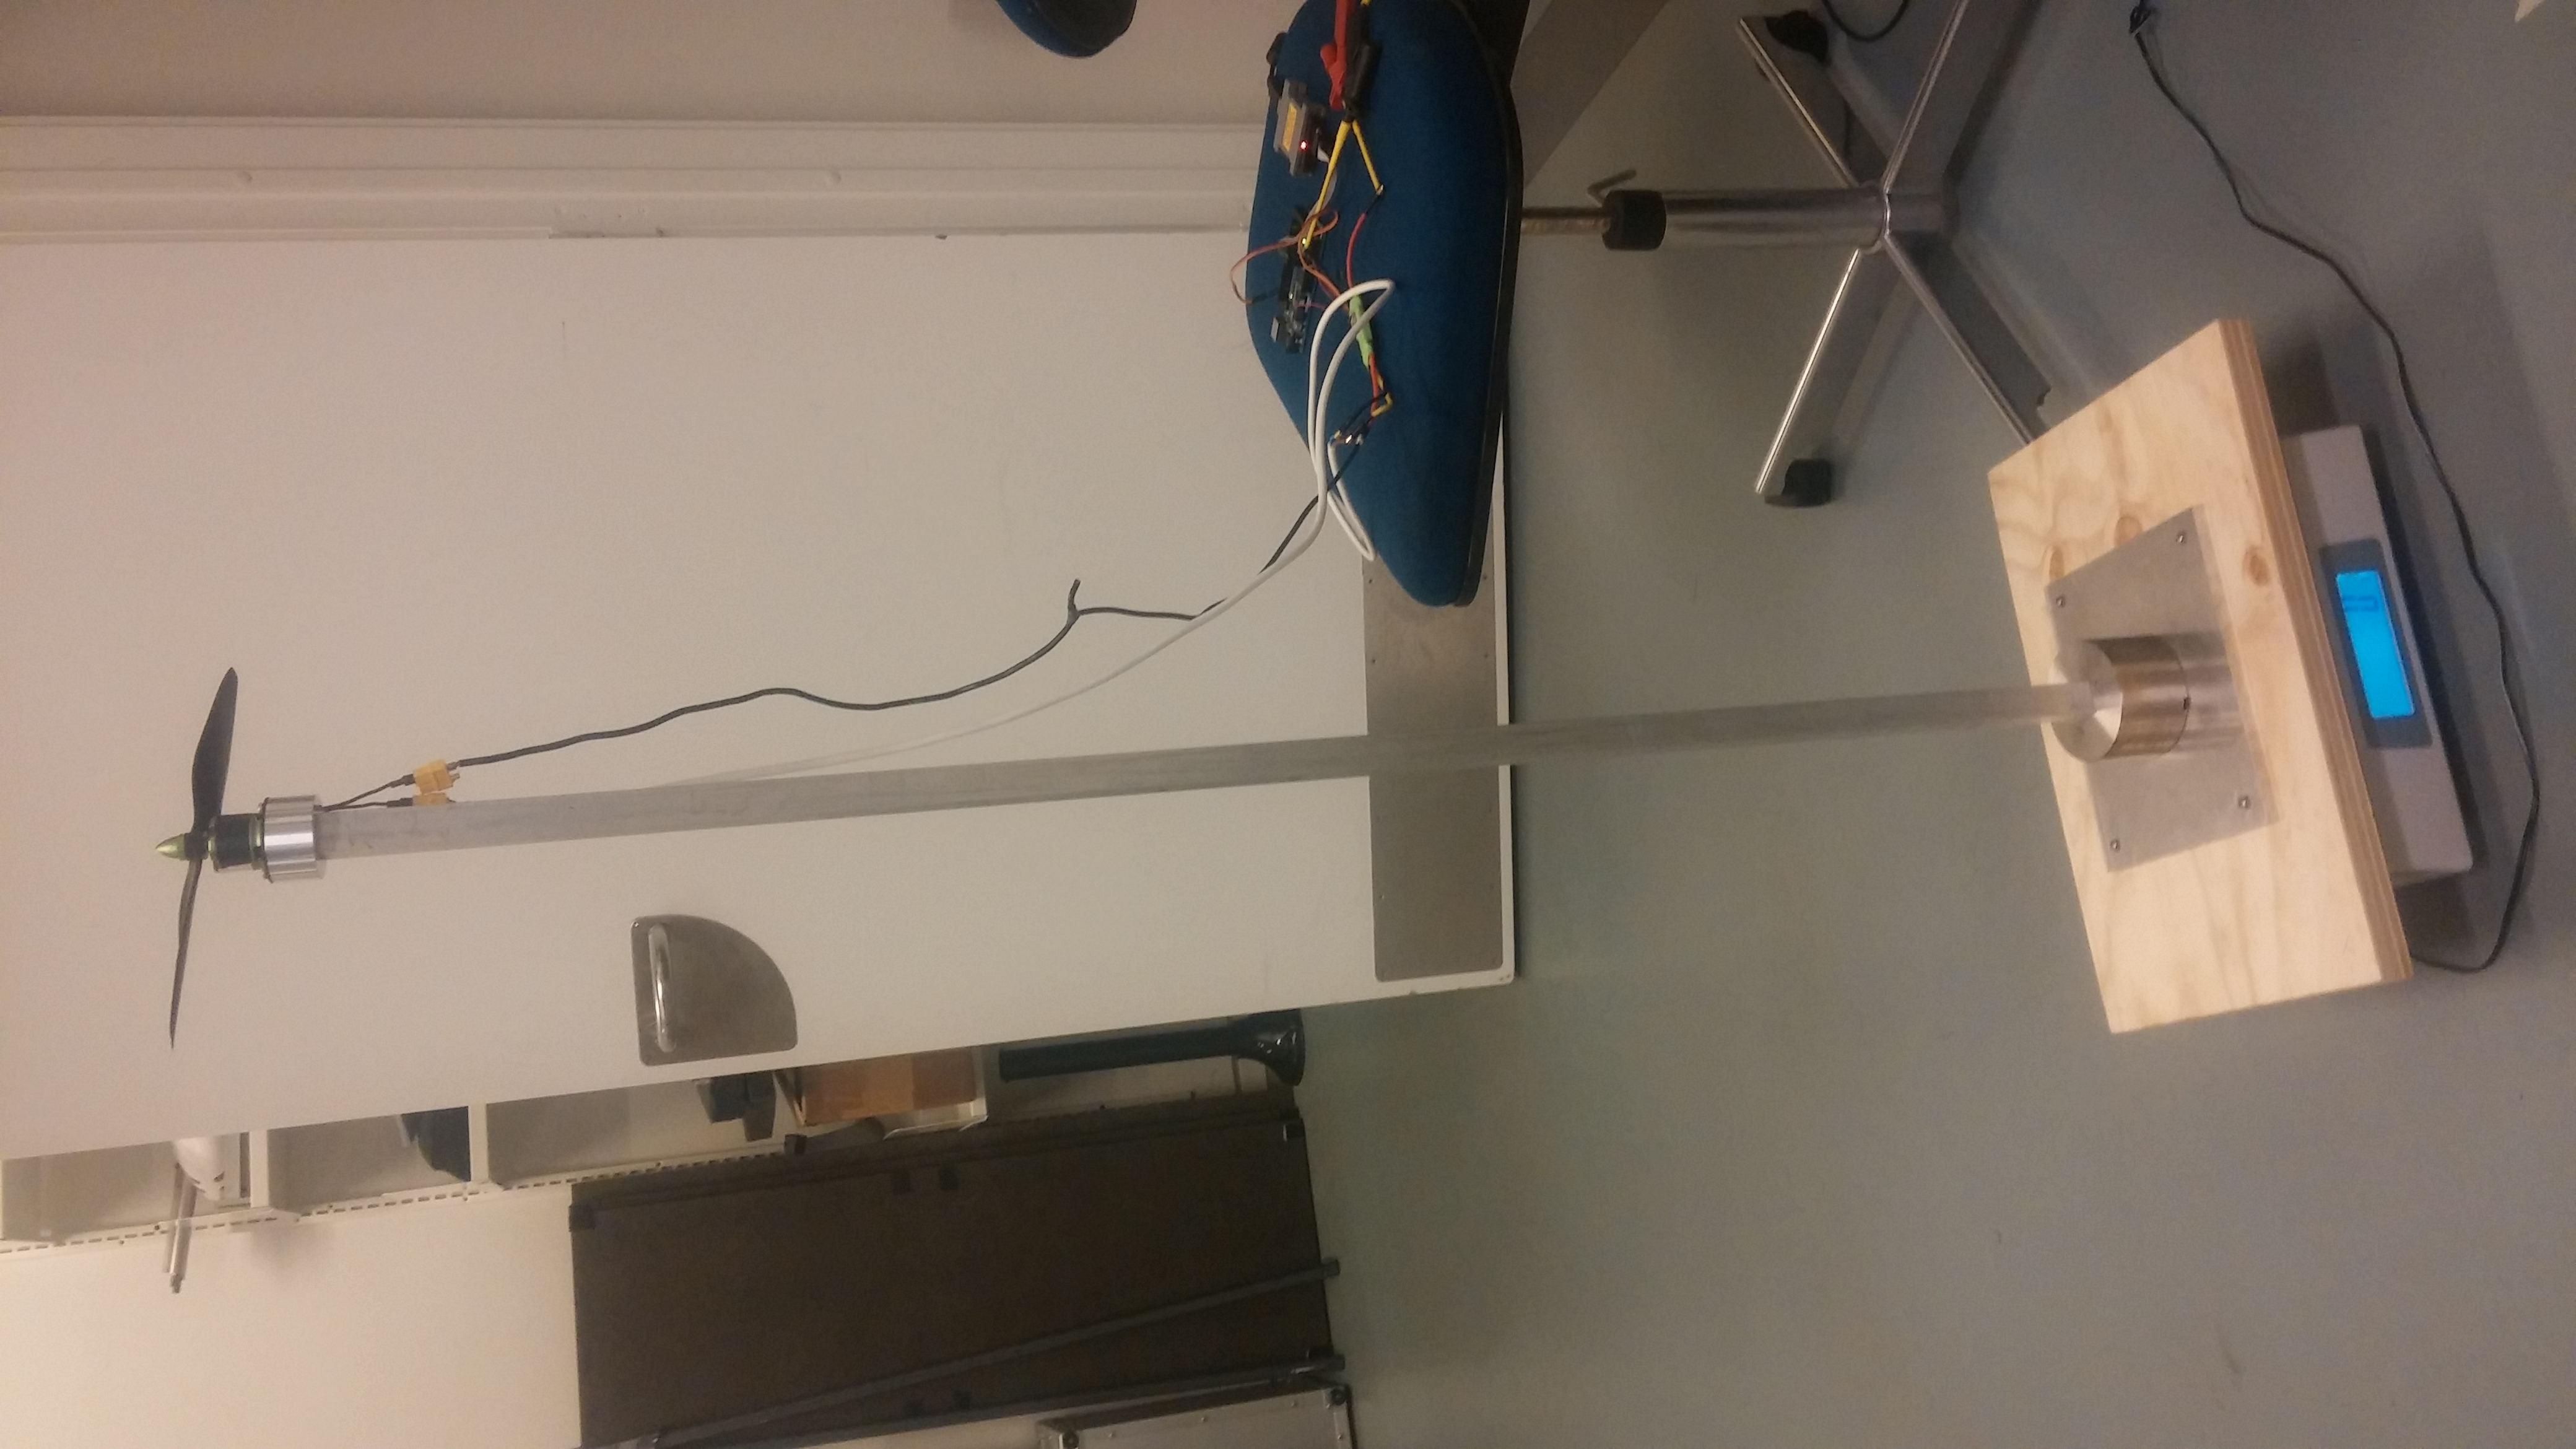
\includegraphics[scale=0.05,angle =-90]{figures/ThrustTestSetup}
	\caption{Setup for the thrust test.}
	\label{ThrustTest}
\end{figure}

\subsubsection{List of Equipment}
\begin{table}[H]
	\begin{tabular}{|l|l|p{4.3cm}|}
		\hline%------------------------------------------------------------------------------------------------------------
		\textbf{Instrument}                                  &  \textbf{AAU-no.}  &  \textbf{Type}                       \\
		\hline%------------------------------------------------------------------------------------------------------------
		Tachometer                                           &  08246           &  Shimpo DT-205		                   \\
		\hline%------------------------------------------------------------------------------------------------------------
	    Power Supply (11.1 V) &  64565                   &  ES 030-5                 \\
		\hline%------------------------------------------------------------------------------------------------------------
		Processing Unit                                   &  N/A               & Arduino Mega     \\
		\hline%------------------------------------------------------------------------------------------------------------
		Motor                                   &  N/A               & Multistar 2213-935     \\
		\hline%------------------------------------------------------------------------------------------------------------
		Motor Speed Controller                                   &  N/A               &  -      \\
		\hline%------------------------------------------------------------------------------------------------------------
		Propeller                                   &  N/A               & Turnigy 1045R     \\
		\hline%------------------------------------------------------------------------------------------------------------
		Scale                                  &  86759              & KERN FCB 12K1     \\
		\hline%------------------------------------------------------------------------------------------------------------
		
	\end{tabular}
\end{table}

\subsubsection{Procedure}
\begin{enumerate}
	\item Construct the setup as seen in \autoref{ThrustTest}, the power supply is connected to the motor driver and the Arduino Mega is powered from the computer. One PWM pin and GND pin from the board must be connected to the driver signal cables yellow and brown respectively. 
	\item Run the program. It should generate a fixed duty PWM signal in the PWM pin.
	\item Wait for the speed to stabilize and read the scale value. The thrust force is calculated by multiplying the added mass in kilograms with the gravitational acceleration (\si{9,81\textbf{ }m/s^2})
	\item Measure the rotational speed with the tachometer.
\end{enumerate}


\subsubsection{Results}
\begin{table}[H]
	\centering
	\begin{tabular}{|l|l|l|l|p{4.3cm}|}
		\hline%------------------------------------------------------------------------------------------------------------
		\textbf{Speed [rpm]}    & \textbf{Speed [rad/s]} & \textbf{Added Mass [g]}  & \textbf{Thrust Force [N]} \\ 
		\hline%------------------------------------------------------------------------------------------------------------
		2240                        	   &  234.57                           & 69                       & 0.68         \\
		\hline%------------------------------------------------------------------------------------------------------------
		2305 						       &  241.38				           & 74                       & 0.73         \\
		\hline%------------------------------------------------------------------------------------------------------------
		2445                               &  256.04   			               & 85                       & 0.83         \\
		\hline%------------------------------------------------------------------------------------------------------------
		2495                               &  261.27			               & 89                       & 0.87         \\
		\hline%------------------------------------------------------------------------------------------------------------
		2585                               &  270.70                          & 97                       & 0.95         \\
		\hline%------------------------------------------------------------------------------------------------------------
		2665 						       &  279.08			           & 99                       & 0.97         \\
		\hline%------------------------------------------------------------------------------------------------------------
		2811                               &  294.36   			           & 114                      & 1.12         \\
		\hline%------------------------------------------------------------------------------------------------------------
		2995                               &  313.63                          & 129                      & 1.27         \\
		\hline%------------------------------------------------------------------------------------------------------------
		3195 						       &  34.57			           & 150                      & 1.47         \\
		\hline%------------------------------------------------------------------------------------------------------------
		3287                               &  344.21  			               & 160                      & 1.57         \\
		\hline%------------------------------------------------------------------------------------------------------------
		3493                               &  365.78                          & 182                      & 1.79         \\
		\hline%------------------------------------------------------------------------------------------------------------
		3609 					           &  377.93	                       & 195                      & 1.91         \\
		\hline%------------------------------------------------------------------------------------------------------------
		3765 						       &  394.26	                   & 215                      & 2.11         \\
		\hline%------------------------------------------------------------------------------------------------------------
		3888 						       &  407.15		                   & 228                      & 2.23         \\
		\hline%------------------------------------------------------------------------------------------------------------
		4060 						       &  425.16	                   & 250                      & 2.46         \\
		\hline%------------------------------------------------------------------------------------------------------------
				
	\end{tabular}
\end{table}
\subsubsection{Results}
The obtained results are shown in \autoref{ThrustGraph}. They have been approximated by a parabolic curve by finding a linear relation between the velocity squared and the thrust force.

\begin{figure}[H]
	\centering
	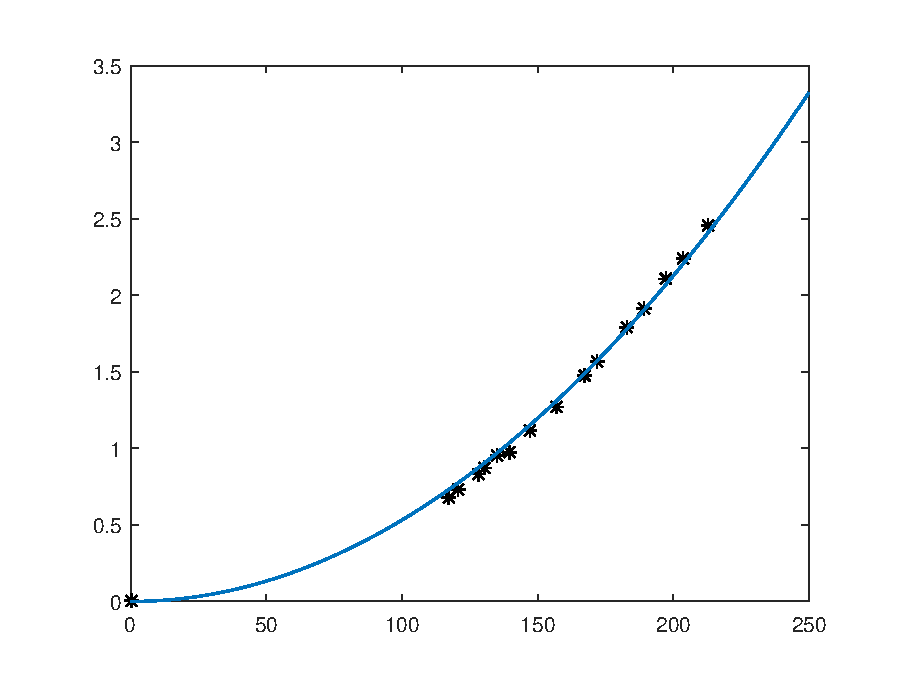
\includegraphics[scale=0.8]{figures/ThrustGraph}
	\caption{Data from the thrust test approximated by a parabolic curve.}
	\label{ThrustGraph}
\end{figure}

The resulting constant that provides the relation between the thrust force in the propeller and the velocity squared is $1.32922\cdot10^{-5} N \cdot s^2 \cdot rad^{-2}$.
